
\documentclass[ms.tex]{subfiles}
\begin{document}

\section{Galactic Properties}
\label{sec:galprops}

\begin{figure*}
\centering
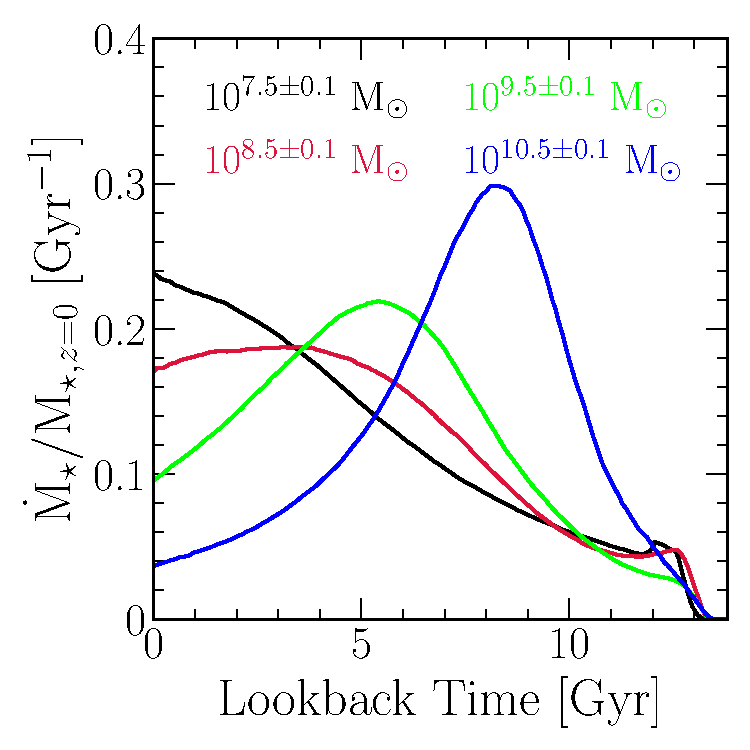
\includegraphics[scale = 0.43]{umachine_sfhs.pdf}
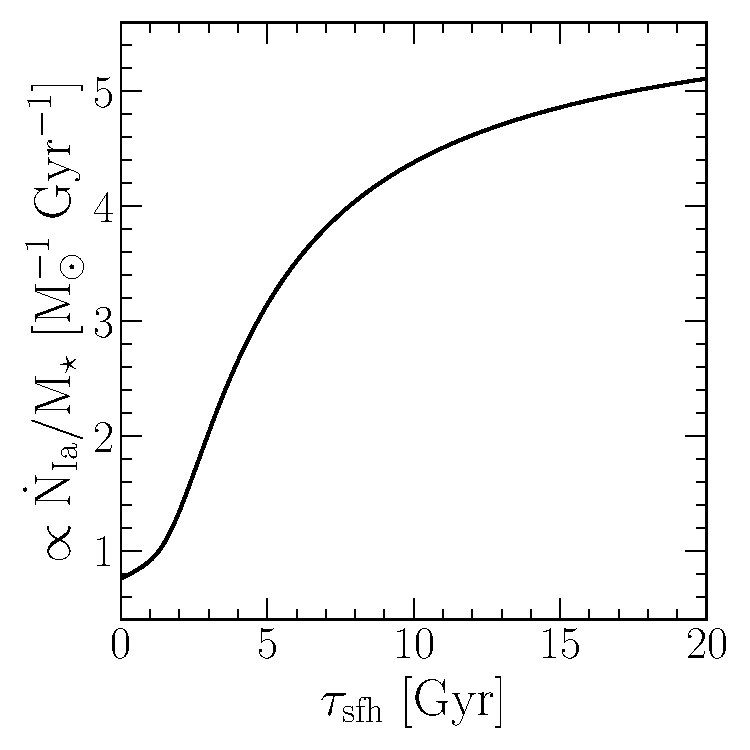
\includegraphics[scale = 0.42]{iarate_vs_tausfh.pdf}
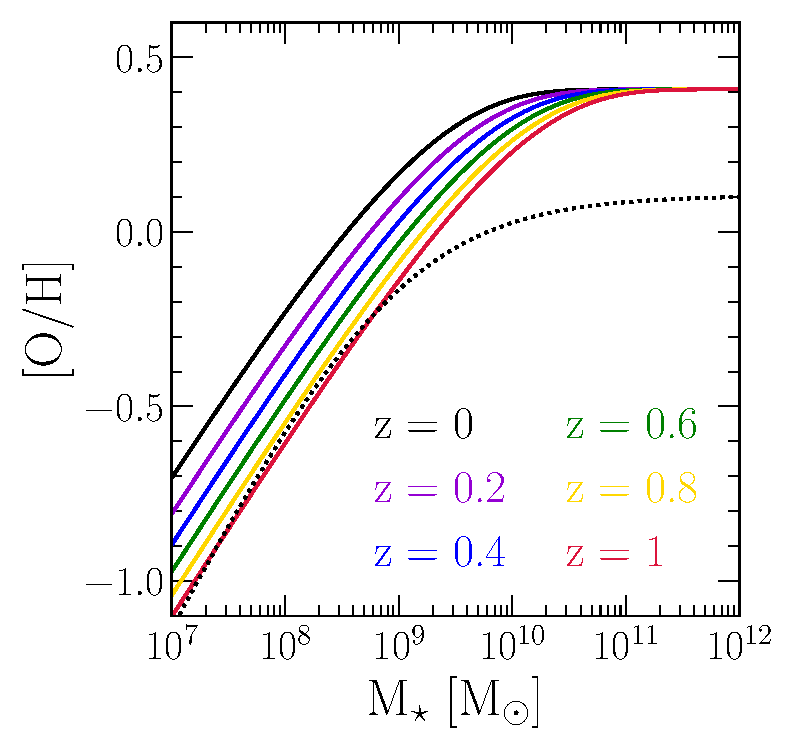
\includegraphics[scale = 0.42]{mzr.pdf}
\caption{Star formation histories.}
\label{fig:sfhs}
\end{figure*}

\subsection{Star Formation Histories}
\label{sec:galprops:sfhs}

\begin{itemize}

	\item We begin by examining how the mean galactic SFH varies with
	present-day stellar mass as predicted by the~\um~SAM of galaxy formation
	\citep{Behroozi2019}.
	Using dark matter halo properties supplied by the~\textit{Bolshoi-Planck}
	and~\textit{Multi-Dark Planck 2} dark matter only simulations
	\citep{Klypin2016, RodriguezPuebla2016},~\um~follows a conventional
	SAM framework (see, e.g., the review in~\citealp{Somerville2015a}),
	parametrizing the SFRs of galaxies as a function of lookback time, the
	assembly history of the halo, and the depth of the halo's potential well.
	Like other SAMs that have come before it,~\um~successfully reproduces a
	broad range of well-constrained observables, including stellar mass
	functions, cosmic SFRs, specific SFRs, quenched fractions, UV luminosity
	functions, and more.
	While previous SAMs have used the extended Press-Schechter formalism
	\citep{Press1974, Bond1991} to generate halo merger trees and push the
	lower stellar mass limit of their model down to
	$M_\star \approx 10^7~\msun$~\citep*[e.g.][]{Somerville2015b}, an advantage
	of~\um~is that the high mass resolution of the~\textit{Bolshoi-Planck} and
	\textit{Multi-Dark Planck 2} simulations allows merger trees down to
	$M_\star = 10^{7.2}~\msun$ to be obtained directly from the simulations.
	This low stellar mass regime is of particular interest to this
	investigation because the~\citet{Brown2019} results on the scaling of the
	specific SN Ia rate with stellar mass reach as low as~$\sim10^7~\msun$ in
	their volume-limited sample and~$\sim10^6~\msun$ in their full sample.

	\item In the left panel of Fig.~\ref{fig:sfhs}, we plot the average SFH as
	a function of lookback time in four narrow bins in observed stellar mass
	taken from~\um.
	In the interest of relating these predictions to data from ASAS-SN, an
	untargeted survey, we take the full galaxy sample from~\um, including both
	star forming and quenched galaxies as well as both centrals and satellites,
	though central galaxies are the dominant population across the full stellar
	mass range.
	In general, low stellar mass galaxies have more extended SFHs than their
	higher mass counterparts.
	This effect is sufficiently strong that around~$M_\star \approx 10^{7.5}
	\msun$, the fastest SFR typically occurs near the present day.
	Unless the SN Ia DTD depends on galaxy mass in a highly peculiar manner,
	this should impact the characteristic SN Ia rate as a function of stellar
	mass.

	\item To illustrate this, we consider a simple qualitative example in which
	the SFH of a galaxy is approximated by a linear-exponential function
	$\dot{M}_\star \propto te^{-t/\tau_\text{sfh}}$.
	For a given DTD~$R_\text{Ia}$ as a function of stellar age~$\tau$, the
	specific SN Ia rate can be expressed as
	\begin{equation}
	\frac{\dot{N}_\text{Ia}}{M_\star} =
	\ddfrac{
		\int_0^{T - t_\text{D}} \dot{M}_\star(\tau) R_\text{Ia}(\tau) d\tau
	}{
		\int_0^T \dot{M}_\star(\tau) d\tau
	},
	\label{eq:specia}
	\end{equation}
	where~$t = T - \tau$ is the time since the onset of star formation,~$T$ is
	the same quantity at the present day, and~$t_\text{D}$ is the minimum delay
	time for a SN Ia event to occur following a single episode of star
	formation.
	% Inspection of the left panel of Fig.~\ref{fig:sfhs} suggests that (on
	% average)~$T \approx 13.2$ Gyr across the full range of stellar masses.
	While the normalization of the SFH cancels, we omit the normalization of
	the DTD from equation~\refp{eq:specia} because we are interested in the
	\textit{relative} scaling of the specific SN Ia rate.
	In~\citet{Brown2019} and~\citet{Gandhi2022}, the rates are normalized to
	the value derived for~$10^{10}~\msun$ galaxies, and we retain the same
	convention here.

	\item Although the details of the SN Ia DTD are a topic of active inquiry
	\citep[e.g.][]{Greggio2005, Strolger2020, Freundlich2021}, comparisons of
	the cosmic SFH~\citep[e.g.][]{Madau2014, Madau2017} with the volumetric SN
	Ia rate as a function of redshift suggest that the cosmic DTD is broadly
	consistent with a~$\tau^{-1}$ power-law (\citealp*{Maoz2012a, Maoz2012b,
	Graur2013};~\citealp{Graur2014}).
	A DTD of approximately this form is also expected under the
	double-degenerate scenario given population synthesis models of binary
	white dwarfs and the loss of angular momentum due to graviational wave
	emission (e.g.~\citealp{Mennekens2010};~\citealp*{Maoz2014}).
	We therefore adopt this parametrization in this paper, though we have
	reconducted our analysis using an exponential DTD with a timescale of
	$\tau_\text{Ia} = 1.5$ Gyr and found similar results.
	% This single power-law is also a common choice in galactic chemical evolution
	% (GCE) models~\citep[e.g.][]{Andrews2017, Johnson2021}, though other simple
	% parametrizations such as an exponential~\citep[e.g.][]{Chen2022} are also
	% common.
	
	\item In principle, the minimum delay of the DTD~$t_\text{D}$ could be as
	short as~$\sim$40 Myr if WDs are produced by~$\lesssim$8~\msun~stars
	\citep*[e.g.][]{Hurley2000}, and perhaps even shorter at low metallicity if
	the total metal content of a star significantly impacts its lifetime as in,
	e.g.,~\citet{Kodama1997} and~\citet{Vincenzo2016}.
	However, if SNe Ia require some additional time following WD formation, the
	minimum delay will be longer.
	Since we are interested in demonstrating the first-order effects of
	variations in SFHs on specific SN Ia rates, we assume a value of
	$t_\text{D} = 100$ Myr, though we note that we have reproduced the results
	in this paper with both~$t_\text{D} = 40$ Myr and~$t_\text{D} = 150$ Myr
	and found similar results in each case.

\end{itemize}

\subsection{The Mass-Metallicity Relation}
\label{sec:galprops:mzr}

\end{document}

